%%Introduction (chpt1)
\section{A brief history of drones}
\Glspl{uav} (Unmanned Aerial Vehicles), more commonly called drones, are defined as flying vehicles without human operators on board. They can be remote-controlled, or controlled by on-board computers. The earliest recorded use of \glspl{uav} dates back to 1849, when Austria launched about 200 unmanned balloons armed with bombs against de city of Venice \cite{anthology}. Due to unfavorable wind conditions, this attack failed, and the experiment was not repeated. The first functional UAVs were made towards de end of World War 1 and their use was, like the Austrian balloons, military. One example is the Kettering Bug (Figure \ref{fig:ketteringbug}), which was a torpedo with wings and a propeller developped by the US Army in 1918 \cite{dronesww1}.
\begin{figure}[H]
  \centering
  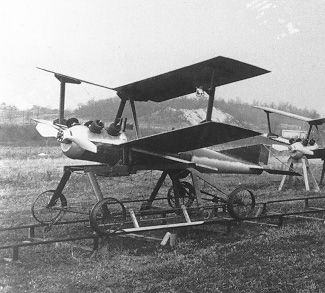
\includegraphics[width=0.5\textwidth]{kettering_bug.jpg}
    \caption{The Kettering Bug (1918)}
    \label{fig:ketteringbug}
\end{figure}

Throughout the 20th century, UAVs become more and more sophisticated, and were used more and more, but always for military purposes. In the more recent years, civilian UAVs have started to appear on the markets and their number quickly exceeded that of military UAVs. In february 2017, the FAA (Federal Aviation Administration) of the United States estimated that around 1.1 million units were in use in the US alone, and expected that number to rise to 3.55 million by 2021 \cite{consumerdronesbythenumbers}. These civilian drones are very different from military drones, in both their form and their function: civilian drones are usually smaller, and use rotors to take off vertically. They are used in a wide variety of applications.

\section{Motivation}
The ability to remote-control small and agile flying objects over large distances through the air, and to bring them to previously inaccessible locations, makes many new things possible. With the increasingly lower prices and better performances of civilian UAVs, people keep finding more and more uses for these high-tech gadgets. Some examples of these applications are: crop monitoring in agriculture \cite{agriculturaldrones}, delivery of mail or parcels, construction \cite{batiravecdesdrones}, cinematography, entertainment, or search and rescue operations. In all these applications, the more autonomous a drone is, the more efficient it will be at its task. One of the main challenges to achieve autonomy is for an UAV to be able to correctly identify its surroundings, and localize itself within them. In outdoor environments, GPS systems allow UAVs to know their position with great accuracy, but this is not possible in GPS-denied environments, such as indoors. The main subject of this thesis will be fully autonomous navigation by a quadcopter in a GPS-denied environment.

\subsection{Ethical considerations}
The new possibilities brought by drones also pose ethical questions about security and privacy. Even though this technology can improve people's quality of life, it also has the potential to diminish it. If drones start to be widely used comercially, we could reach a point where the sound nuisances that they cause seriously impacts people who live in densely populated areas. Also, they can make us feel less at home, knowing that we could be observed from the sky. For this reason, it is important to adopt strict reulations regarding the use of drones in public spaces. Fortunately, many countries are already adopting legislation in this direction.


\section{Context}
This thesis is part of a project at the UCL that spans over several years and several masters theses. This project was launched by professor Julien Hendrickx in the 2012-2013 academic year, and had as long-term goal to develop a program that would enable low-cost UAVs to navigate autonomously in indoor environments. This means creating a map of their environment, localizing themselves in this map, and avoidig obstacles during exploration, using only on-board sensors. Another goal is to allow several drones to collaborate to speed up exploration. Five theses have already been written on this subject, each taking the work of the previous a little further.
\paragraph{2012-2015: First three theses}
In each of the three academic years (2012-2013, 2013-2014, 2014-2015), one masters thesis on the subject of indoor navigation for autonomous low-cost drones was written. These masters theses formed the base of the future work. They implemented visual SLAM methods to allow drones to build a two-dimensional map based on keypoints (first red pucks, then visual landmarks that the drone detected from a textured field of view), and to localize itself within this map. During this time, inter-drone communication was also established, and was used to allow a drone to communicate the location of a target to another drone.

\paragraph{2015-2016: Recent work}
Last year, two groups of students simultaneously wrote theses on this subject. Before doing so, they joined forces to reimplement what had been done previously, but using the ROS interface, an interface to work with robots that would make many things simpler, and allow more flexibility (see section %%TODO for more).
The work of the first group of students allowed a drone to search and follow a mobile target, and call a second drone to continue this task when its battery was low.\\
The second group of students extended to SLAM algorithm to allow to use a 3D map to localize the drone. Unfortunately, they did not implement triangulation to allow to project seen points into 3D space, but rather made the assumption that all points were located on the ground when building the map. The end result was a drone capable of using a 3D map to localize itself, but not capable of building one from its observations.


\section{Objectives}
For my own thesis, my goal is to continue the work of last year's second group, to allow true 3-D SLAM: to build a 3D map based on observations by the monocular camera. To achieve this goal I will follow the following steps:
\begin{itemize}
\item Research the current state of the art for 3D Keyframe based monocular visual SLAM
\item Implement a way to triangulate points based on observations
\item Bundle Adjustment
\item Dense reconstruction
\item Obstacle Avoidance
\end{itemize}

\section{Structure}
%TODO after the rest is done
